Multi-armed bandits represent the simplest form of reinforcement learning: sequential decision-making without state. The agent repeatedly chooses among $K$ actions, observes a stochastic reward, and updates its beliefs. This stateless structure makes bandits uniquely suited for real-world deployment where the cost of suboptimal decisions is immediate and irreversible. The central challenge is the exploration-exploitation tradeoff: the agent must balance gathering information about uncertain arms against exploiting arms that appear best. Two algorithmic paradigms dominate. The Gittins index, derived from dynamic programming under discounting, provides the Bayes-optimal solution for independent arms but requires solving a stopping problem for each arm at each period.\footnote{\citet{Gittins1979} showed that the optimal policy for the discounted infinite-horizon bandit has an index form: compute a scalar index for each arm based on its posterior, then pull the arm with highest index. The index equals the fair subsidy that makes the agent indifferent between pulling the arm and receiving a guaranteed payment.} Upper Confidence Bound (UCB) algorithms offer a frequentist alternative with finite-time regret guarantees and minimal computational overhead. This chapter explores how economic structure improves upon generic bandit algorithms. When the reward function satisfies monotonicity, unimodality, or revealed preference constraints from consumer theory, algorithms can eliminate suboptimal arms faster and achieve logarithmic rather than square-root regret scaling.

A $K$-armed bandit is an MDP with a single state. The action set is $\mathcal{A} = \{1, \ldots, K\}$, and pulling arm $a$ yields reward $r_t \sim \nu_{a}$ with mean $\mu_{a}$.\footnote{Formally, $|\mathcal{S}| = 1$, so there is no state transition or discounting. Unlike full RL which runs in simulation, bandits deploy in real-time where sample efficiency is critical.} The standard metric is regret:
\[
R(T) = T \cdot \max_i \mu_i - \mathbb{E}\left[\sum_{t=1}^T r_t\right].
\]
Regret measures the profit lost due to not knowing the optimal arm. Standard algorithms achieve $O(\sqrt{KT})$ regret. Economic structure can improve this to $O(\log T)$.

\subsection{Dynamic Pricing with Demand Learning}

A seller faces sequential customers with unknown demand. Setting price $p \in \mathcal{P} = \{p_1, \ldots, p_K\}$ yields sale probability $\theta(p)$ and revenue $R_t = p \cdot \mathbb{1}\{\text{sale}\}$. Microeconomic theory provides structure: $\theta(p)$ decreases monotonically in $p$.\footnote{Consumers purchase when valuation exceeds price. If valuations follow distribution $F$, then $\theta(p) = 1 - F(p)$.} Under the monotone hazard rate condition,\footnote{The hazard rate of distribution $F$ is $h(v) = f(v)/(1-F(v))$. The monotone hazard rate (MHR) condition requires $h(v)$ to be non-decreasing. Many common distributions (uniform, exponential, normal) satisfy MHR. Under MHR, revenue $p(1-F(p))$ is strictly quasi-concave, ensuring a unique optimal price.} expected revenue $\mu(p) = p \cdot \theta(p)$ is unimodal.

\citet{Misra2019} exploit unimodality with a modified UCB algorithm\footnote{Upper Confidence Bound (UCB) algorithms balance exploration and exploitation by selecting the arm with highest upper confidence bound $\hat{\mu}_a + c\sqrt{\ln t / N_a}$, where $\hat{\mu}_a$ is the empirical mean, $N_a$ the number of pulls, and $c$ controls the exploration bonus. Arms with high uncertainty or high estimated reward receive priority.} that maintains a leader arm and explores only the leader and its neighbors:
\begin{equation}
I_p(t) = \hat{\mu}_p(t) + \sqrt{\frac{2\ln t}{N_p(t)}}
\end{equation}
where $\hat{\mu}_p(t)$ is average revenue and $N_p(t)$ the number of trials at price $p$. When a neighbor's index exceeds the leader's, the algorithm shifts focus. This achieves $O(\log T)$ profit loss versus $O(\sqrt{KT})$ for standard UCB.\footnote{Field experiments at an online retailer showed 43\% higher profits versus static pricing.} We implement this algorithm in Section~\ref{sec:bandit_sim}.

For multi-product settings, \citet{Mueller2019} impose low-rank structure on the price-sensitivity matrix $\mathbf{B}$ in the demand system $\mathbf{q}_t = \mathbf{c}_t - \mathbf{B}\mathbf{p}_t + \boldsymbol{\varepsilon}_t$, achieving profit loss $O(T^{3/4}\sqrt{d})$ scaling with latent dimension $d \ll N$.\footnote{\citet{Xu2021} achieve $O(d \log T)$ for contextual pricing with linear valuations $v_t = \boldsymbol{\theta}^\top \mathbf{x}_t$. \citet{Goyal2022} handle MNL choice models (multinomial logit extends the binary logit to $K > 2$ alternatives; in pricing, MNL models consumer choice among differentiated products where utility depends on product attributes and price), achieving $O(d\sqrt{T}\log T)$ under adversarial contexts.}

\subsection{Bid Optimization in Auctions}

In a second-price auction\footnote{In a second-price (Vickrey) auction, bidders submit sealed bids and the highest bidder wins, paying the second-highest bid. This mechanism is incentive-compatible: bidding one's true valuation is a weakly dominant strategy regardless of others' behavior.} with reserve $r$, revenue is $b_{(2)}\mathbb{1}\{b_{(2)} > r\} + r\mathbb{1}\{b_{(1)} \geq r > b_{(2)}\}$. Myerson's theory establishes that expected revenue is unimodal in $r$ under regularity conditions.\footnote{\citet{myerson1981} shows the optimal reserve price satisfies $r^* = \psi^{-1}(0)$ where $\psi(v) = v - (1-F(v))/f(v)$ is the virtual valuation. Regularity requires $\psi(v)$ to be strictly increasing, which holds under the MHR condition.} \citet{CesaBianchi2015} leverage this with a unimodal bandit algorithm, achieving $O(\log T)$ profit loss by eliminating provably suboptimal regions.\footnote{\citet{Akcay2022} address censored feedback where losing bids are unobserved, using auction rules to convert partial observations into side information.}

\subsection{Strategic Interactions}

\citet{Guo2023} study multi-firm pricing where consumers follow a logit model\footnote{The logit (multinomial logit) model specifies choice probabilities as $\Pr(\text{choose } i) = e^{U_i}/\sum_j e^{U_j}$, where $U_i$ is the utility of option $i$. It derives from assuming i.i.d.\ Type-I extreme value (Gumbel) errors $\epsilon_{i,t}$. The model implies the independence of irrelevant alternatives (IIA) property.} with reference price effects:\footnote{Reference price effects capture the behavioral finding that consumers evaluate prices relative to an anchor. The reference price $\rho_t$ represents the expected price level; a current price below $\rho_t$ feels like a gain, boosting purchase probability beyond what absolute price alone would predict.}
\begin{equation}
U_t(i) = \alpha_i - \beta p_{i,t} + \gamma(\rho_t - p_{i,t}) + \epsilon_{i,t}, \quad \rho_{t+1} = (1-\delta)\rho_t + \frac{\delta}{n}\sum_i p_{i,t}
\end{equation}
Online projected gradient ascent achieves $O(1/t)$ convergence to Nash equilibrium, faster than model-free approaches.

\subsection{Simulation Study: Dynamic Pricing with Partial Identification}
\label{sec:bandit_sim}

We replicate the simulation of \citet{Misra2019} to evaluate UCB-PI against standard bandit algorithms. The environment has $K = 100$ prices on a grid from \$0.01 to \$1.00, $S = 1{,}000$ consumer segments with equal weights, and within-segment heterogeneity $\delta = 0.1$. Each segment $s$ has midpoint valuation $v_s \sim \mathrm{Uniform}(0.1, 0.9)$, and consumer $i$ in segment $s$ has valuation $v_i \sim \mathrm{Uniform}(v_s - \delta, v_s + \delta)$. A consumer purchases if and only if $v_i \geq p$ (WARP). The optimal price is $p^* = 0.45$ with expected profit $\mu^* = 0.248$ per customer. We run $T = 200{,}000$ rounds across 10 seeds.

We compare five algorithms spanning the model-free to model-based spectrum. Table~\ref{tab:algorithm_class} summarizes their theoretical properties. UCB1 is the standard upper confidence bound algorithm with no structural assumptions. Thompson Sampling maintains Beta posteriors over arm means and samples to select actions. Learn-Then-Exploit (LTE) uses a pure exploration phase followed by greedy exploitation. UCB-PI incorporates the partial identification mechanism of \citet{Misra2019}, eliminating dominated prices using WARP bounds. UCB-PI-tuned uses a more conservative dominance threshold ($2\delta$ vs.\ $\delta$) to reduce false eliminations.

\begin{table}[!htbp]
\centering
\caption{Algorithm classification by structure exploitation. Regret rates are theoretical under standard assumptions; $K$ is the number of arms, $T$ the horizon.}
\label{tab:algorithm_class}
\begin{tabular}{lccc}
\toprule
Algorithm & Uses WARP & Uses Unimodality & Regret Rate \\
\midrule
UCB1 & No & No & $O(\sqrt{KT})$ \\
Thompson & No & No & $O(\sqrt{KT})$ \\
LTE (5\%) & No & No & $O(T^{2/3})$ \\
UCB-PI & Yes & Implicit & $O(\log T)$ \\
UCB-PI-tuned & Yes & Implicit & $O(\log T)$ \\
\bottomrule
\end{tabular}
\end{table}

Table~\ref{tab:bandit_results} reports cumulative profits and ex-post profit ratios. UCB-PI-tuned achieves the highest mean profit ratio at 99.4\%, followed by Thompson Sampling at 97.9\%. The partial identification mechanism eliminates dominated prices: by $T = 200{,}000$, UCB-PI has eliminated 37 of 100 prices on average, while UCB-PI-tuned eliminates 15.

\begin{table}[!htbp]
\centering
\caption{Dynamic pricing with partial identification ($K = 100$ prices, $S = 1{,}000$ segments, $T = 200{,}000$ customers, 10 seeds). Frac.\ Opt is the fraction of rounds at $p^*$. Dominated is mean number of prices eliminated by partial identification.}
\label{tab:bandit_results}
\begin{tabular}{lcccccc}
\toprule
Algorithm & Ex Post \% & Range & Profit & Frac.\ Opt & Dominated \\
\midrule
Oracle & 100.0\% & [100-100\%] & 50701 & 0.200 & -- \\
UCB-PI-tuned & 99.4\% & [99-100\%] & 50387 $\pm$ 658 & 0.104 & 15 \\
UCB-PI & 92.4\% & [91-93\%] & 46831 $\pm$ 724 & 0.048 & 37 \\
UCB1 & 86.8\% & [86-87\%] & 44024 $\pm$ 597 & 0.028 & -- \\
LTE (5\%) & 95.6\% & [92-98\%] & 48510 $\pm$ 1123 & 0.000 & -- \\
Thompson & 97.9\% & [98-98\%] & 49634 $\pm$ 657 & 0.094 & -- \\
\bottomrule
\end{tabular}

\end{table}

Figure~\ref{fig:bandit_profit} shows cumulative profit trajectories. All learning algorithms converge toward oracle performance, with UCB-PI-tuned tracking the oracle most closely throughout.

\begin{figure}[!htbp]
\centering
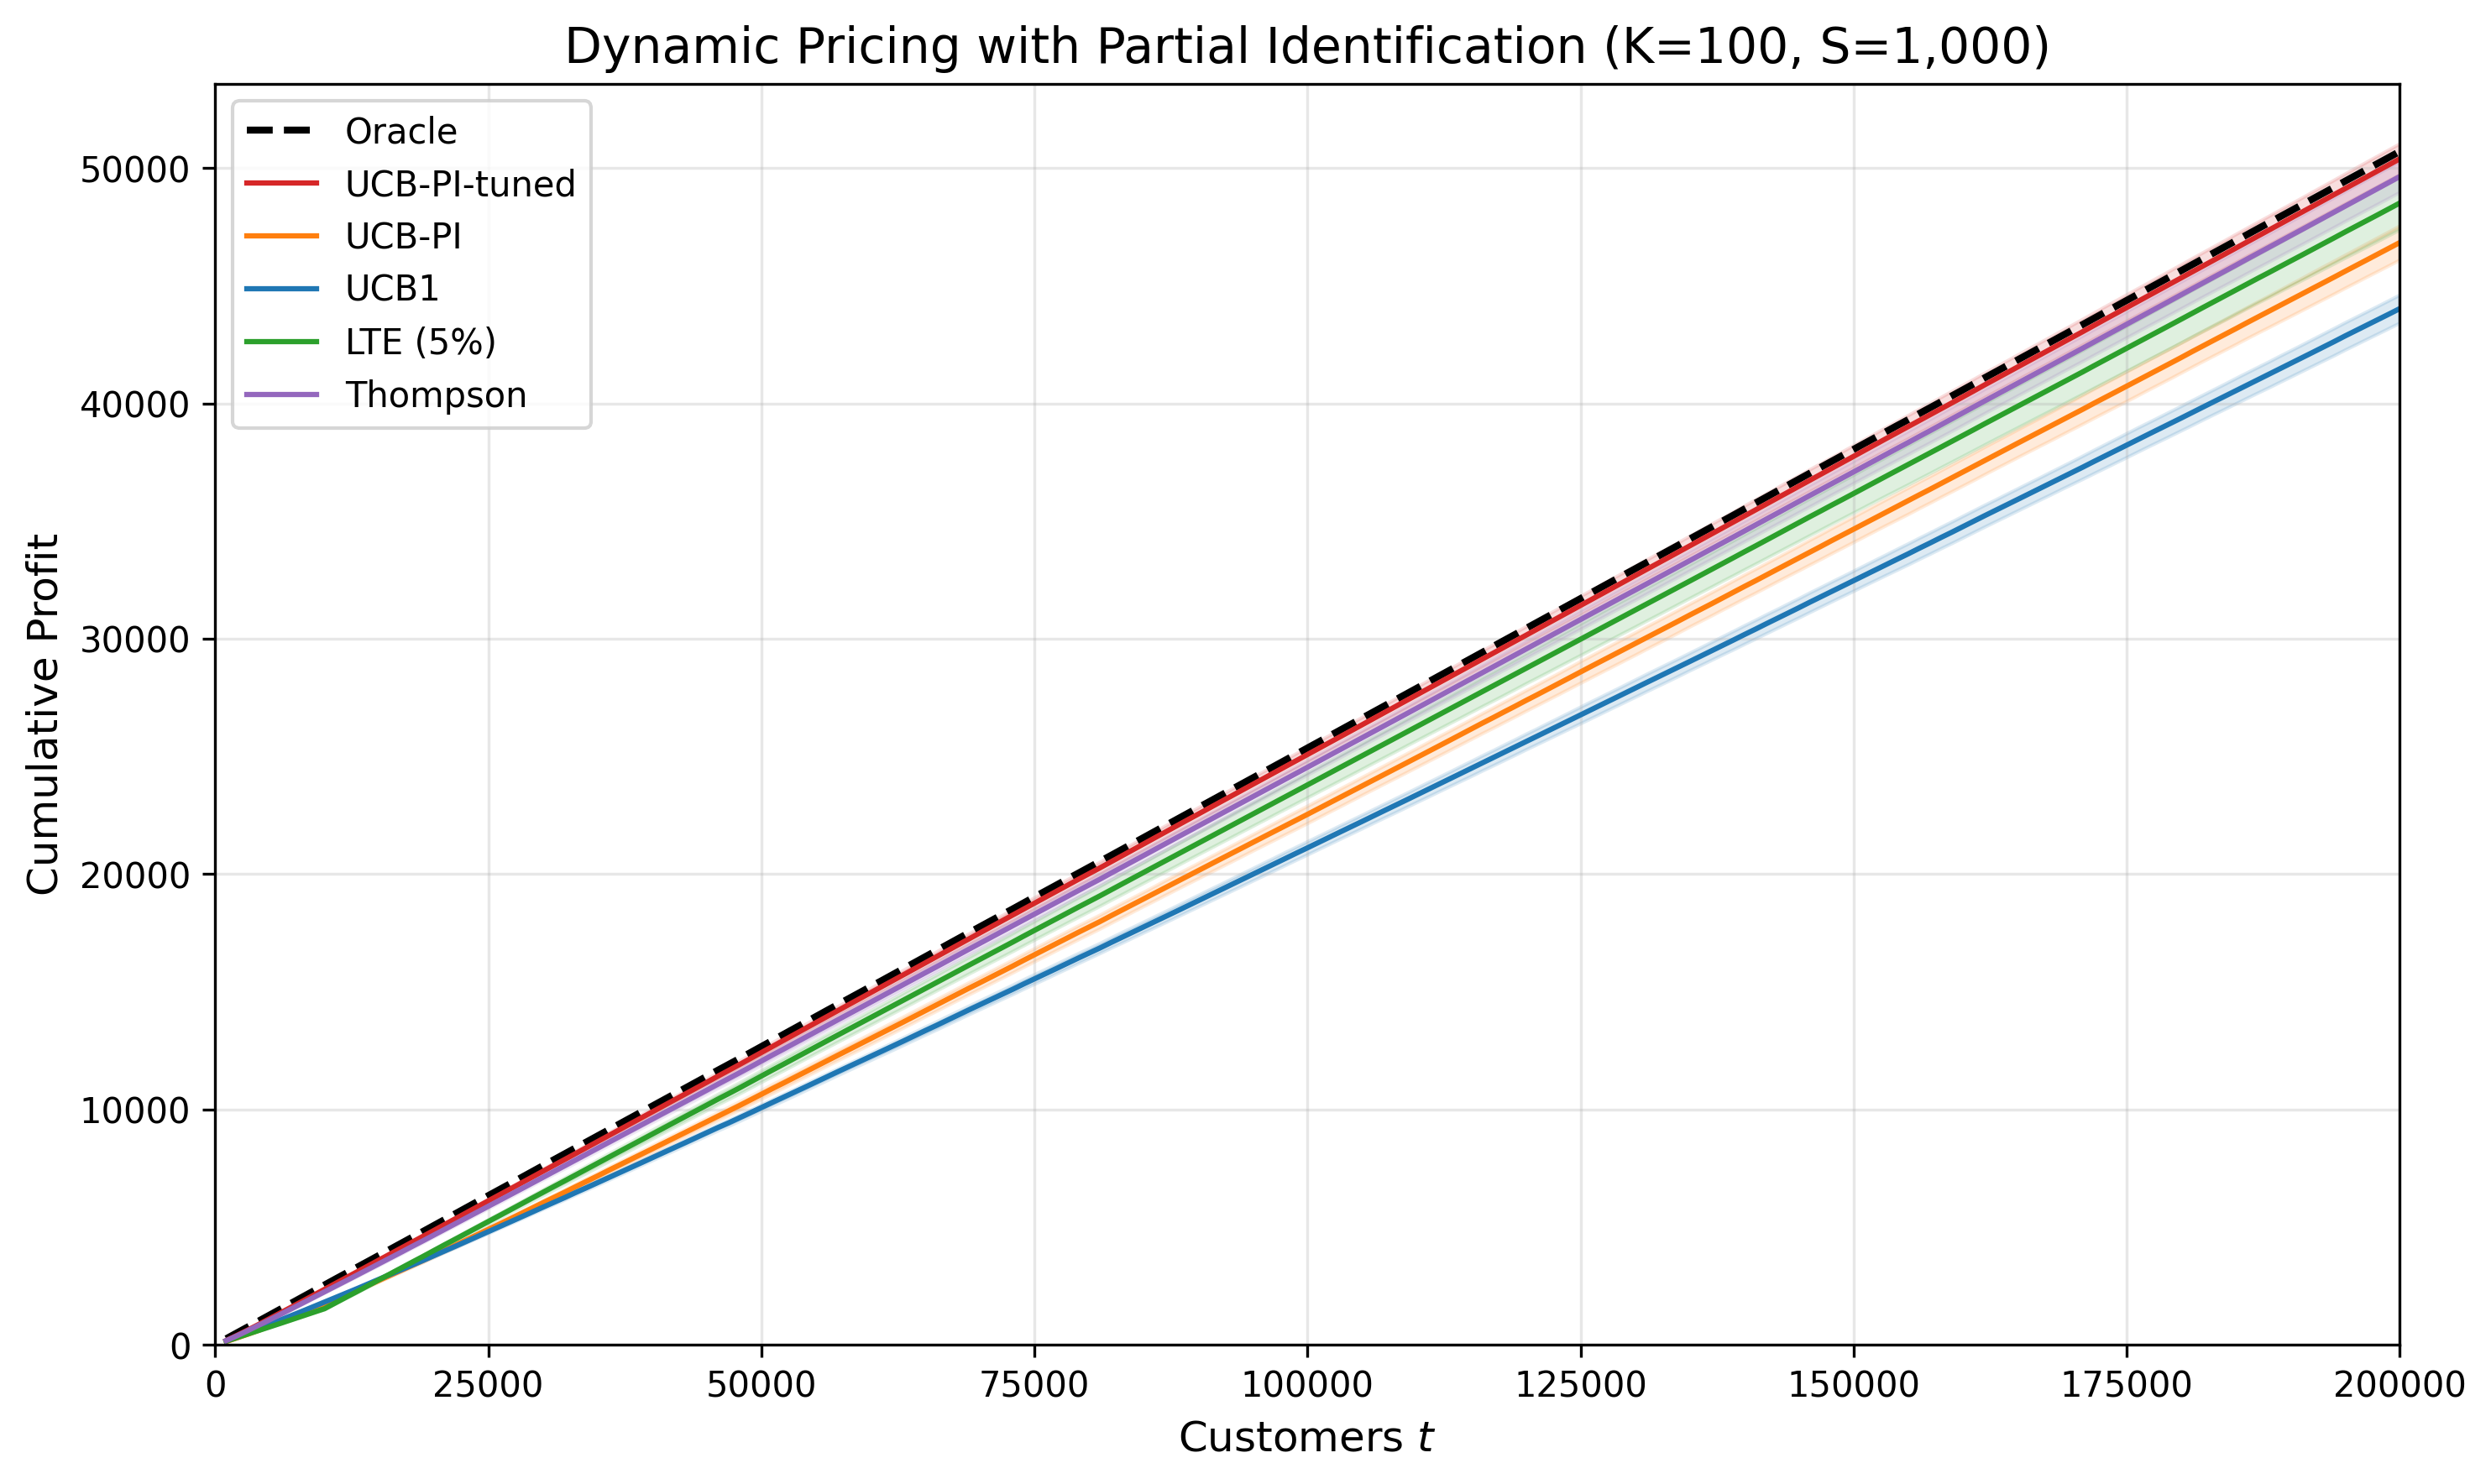
\includegraphics[width=0.9\textwidth]{../ch06_bandits/sims/structural_pricing_misra_profit.png}
\caption{Cumulative profit for dynamic pricing with partial identification. Oracle (dashed black) knows demand perfectly. Shaded regions show $\pm 2$ standard errors across 10 seeds.}
\label{fig:bandit_profit}
\end{figure}

Figure~\ref{fig:regret_scaling} validates the theoretical regret rates. When regret is divided by $\log(t)$, algorithms with $O(\log T)$ regret should stabilize while $O(\sqrt{T})$ algorithms diverge. UCB-PI-tuned stabilizes near 26, consistent with logarithmic regret. UCB1 and Thompson grow without bound, consistent with $O(\sqrt{T})$. UCB-PI shows intermediate behavior: the dominance mechanism reduces regret but overly aggressive elimination (37 prices dominated vs.\ 15 for tuned) causes some suboptimality.

\begin{figure}[!htbp]
\centering
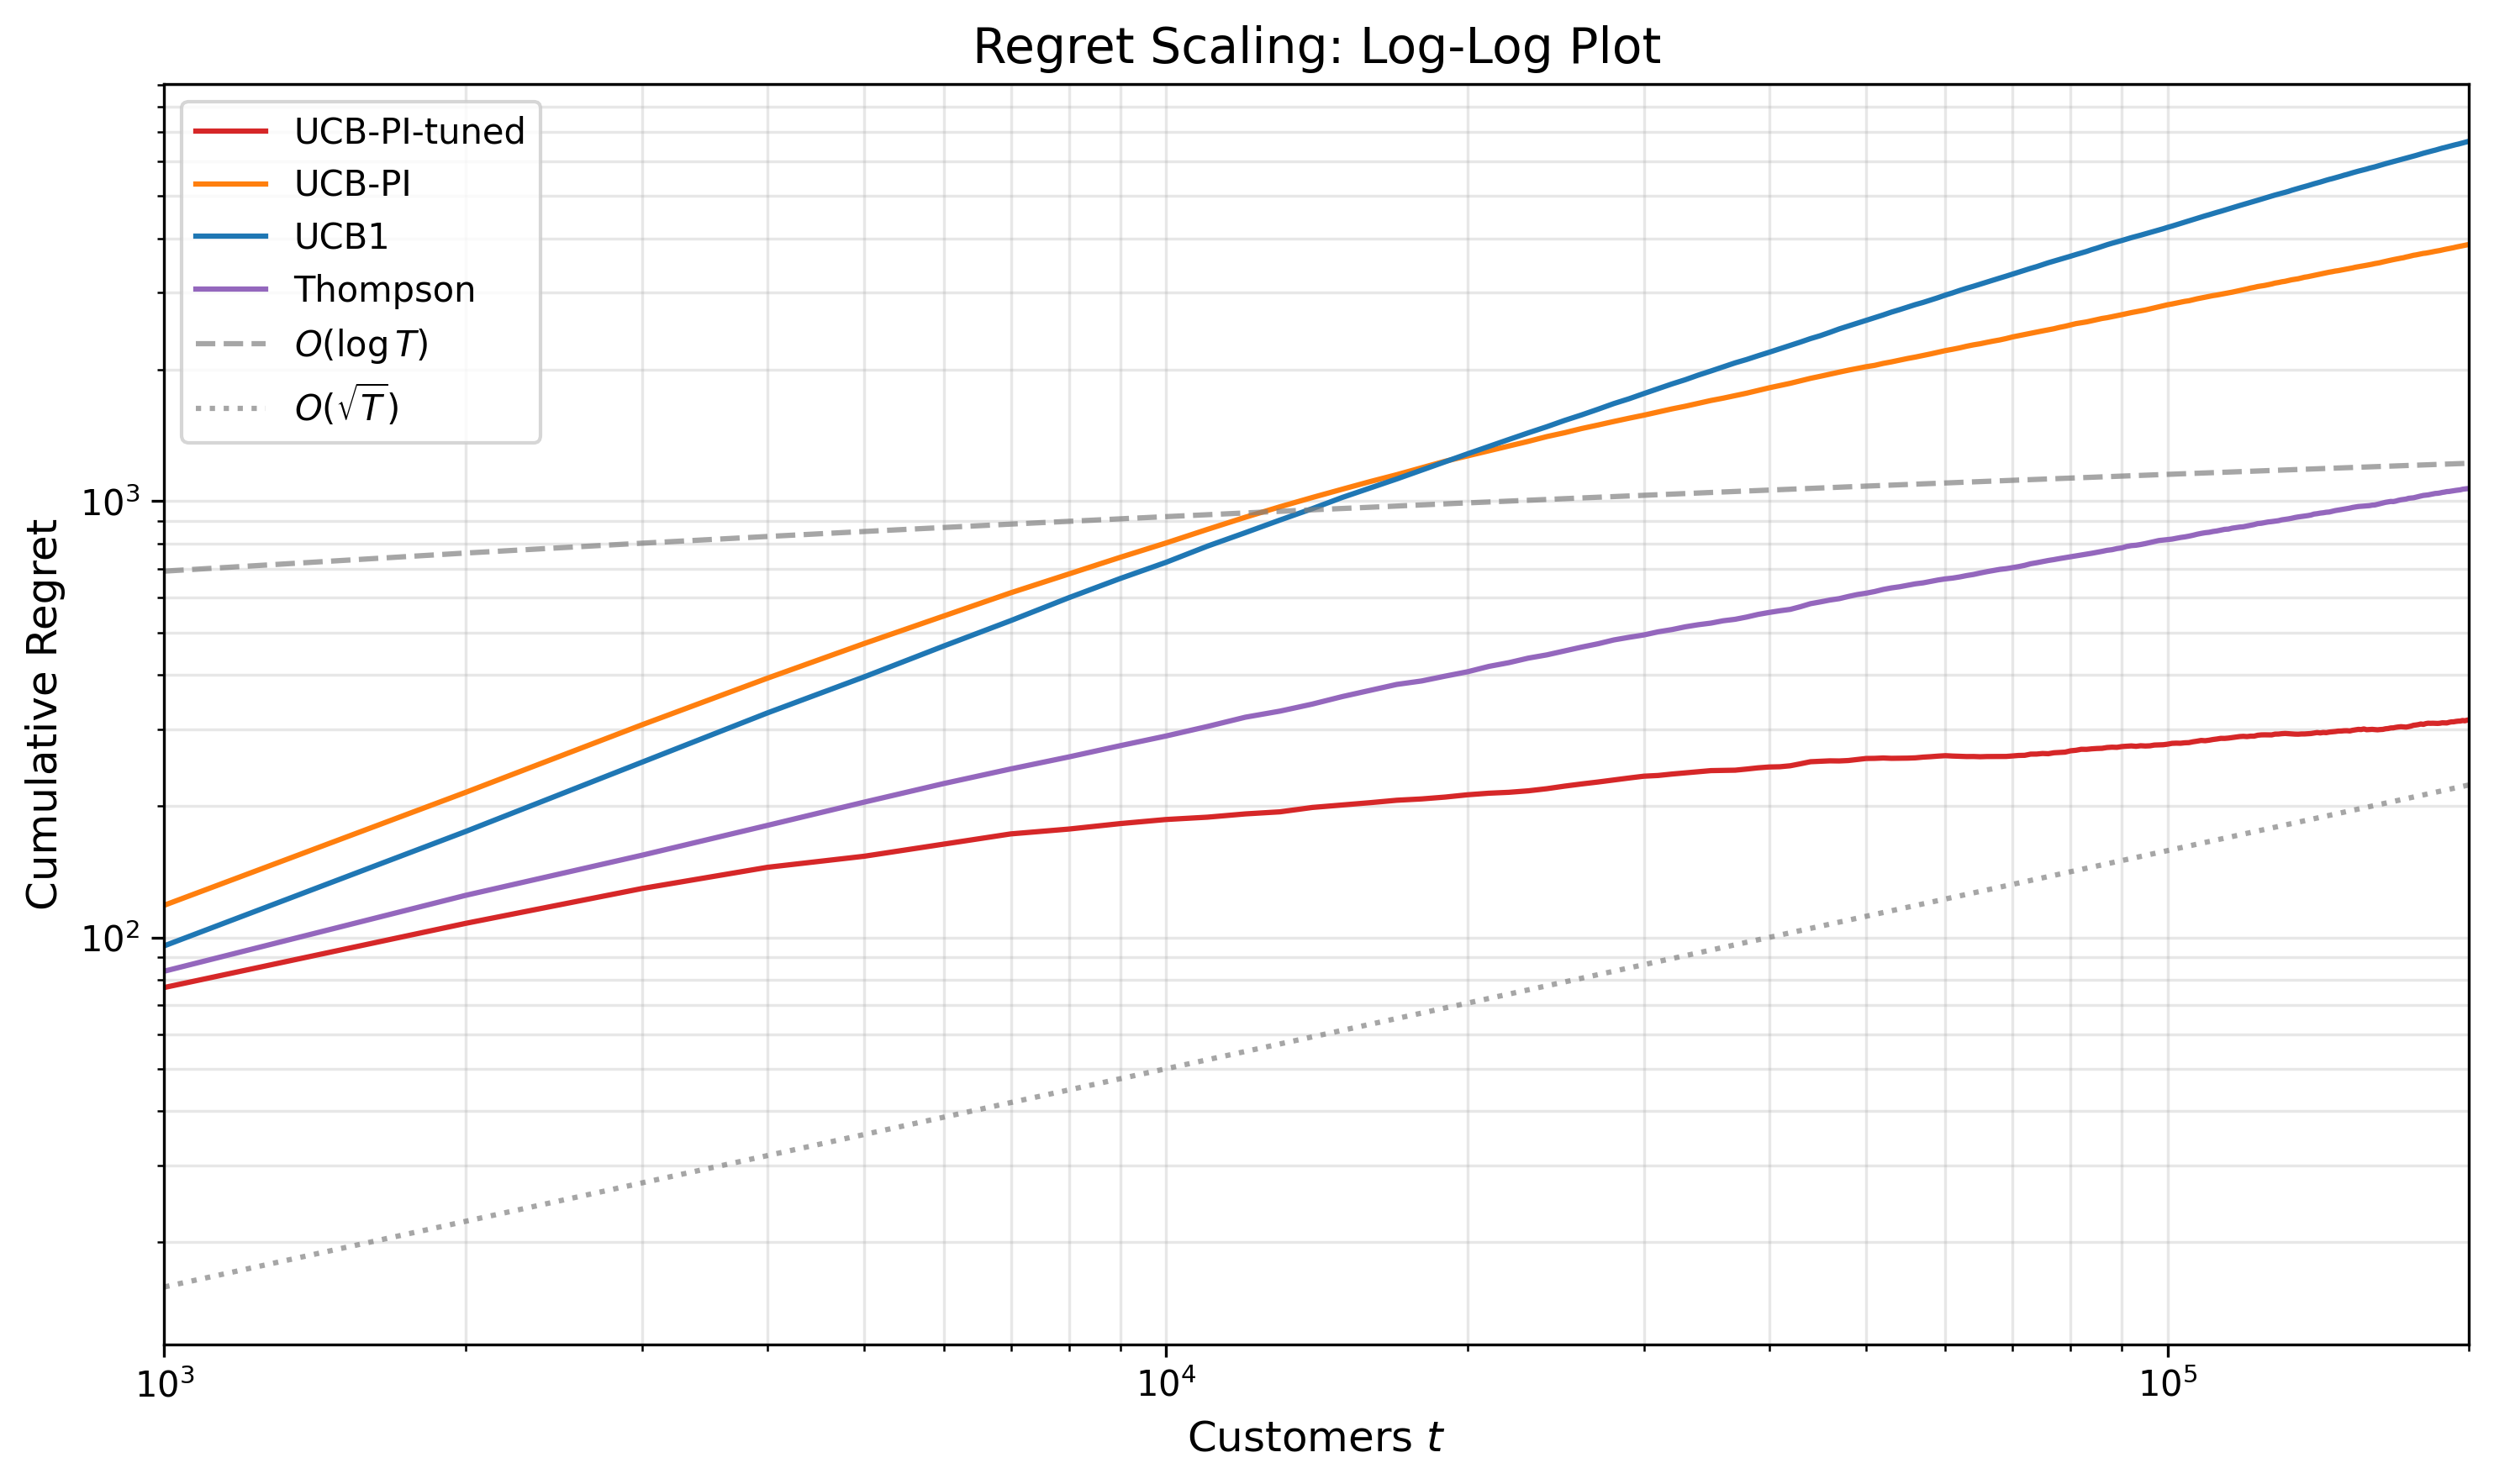
\includegraphics[width=0.9\textwidth]{../ch06_bandits/sims/structural_pricing_misra_regret_scaling.png}
\caption{Regret scaling validation. Profit loss divided by $\log(t)$ should stabilize for $O(\log T)$ algorithms and grow for $O(\sqrt{T})$ algorithms.}
\label{fig:regret_scaling}
\end{figure}

Figure~\ref{fig:price_histogram} shows the distribution of price selections across the horizon. UCB-PI-tuned concentrates selections around the optimal price $p^* = 0.45$, with the distribution tightening as more prices are eliminated. UCB1 spreads selections more broadly, reflecting continued exploration across all arms.

\begin{figure}[!htbp]
\centering
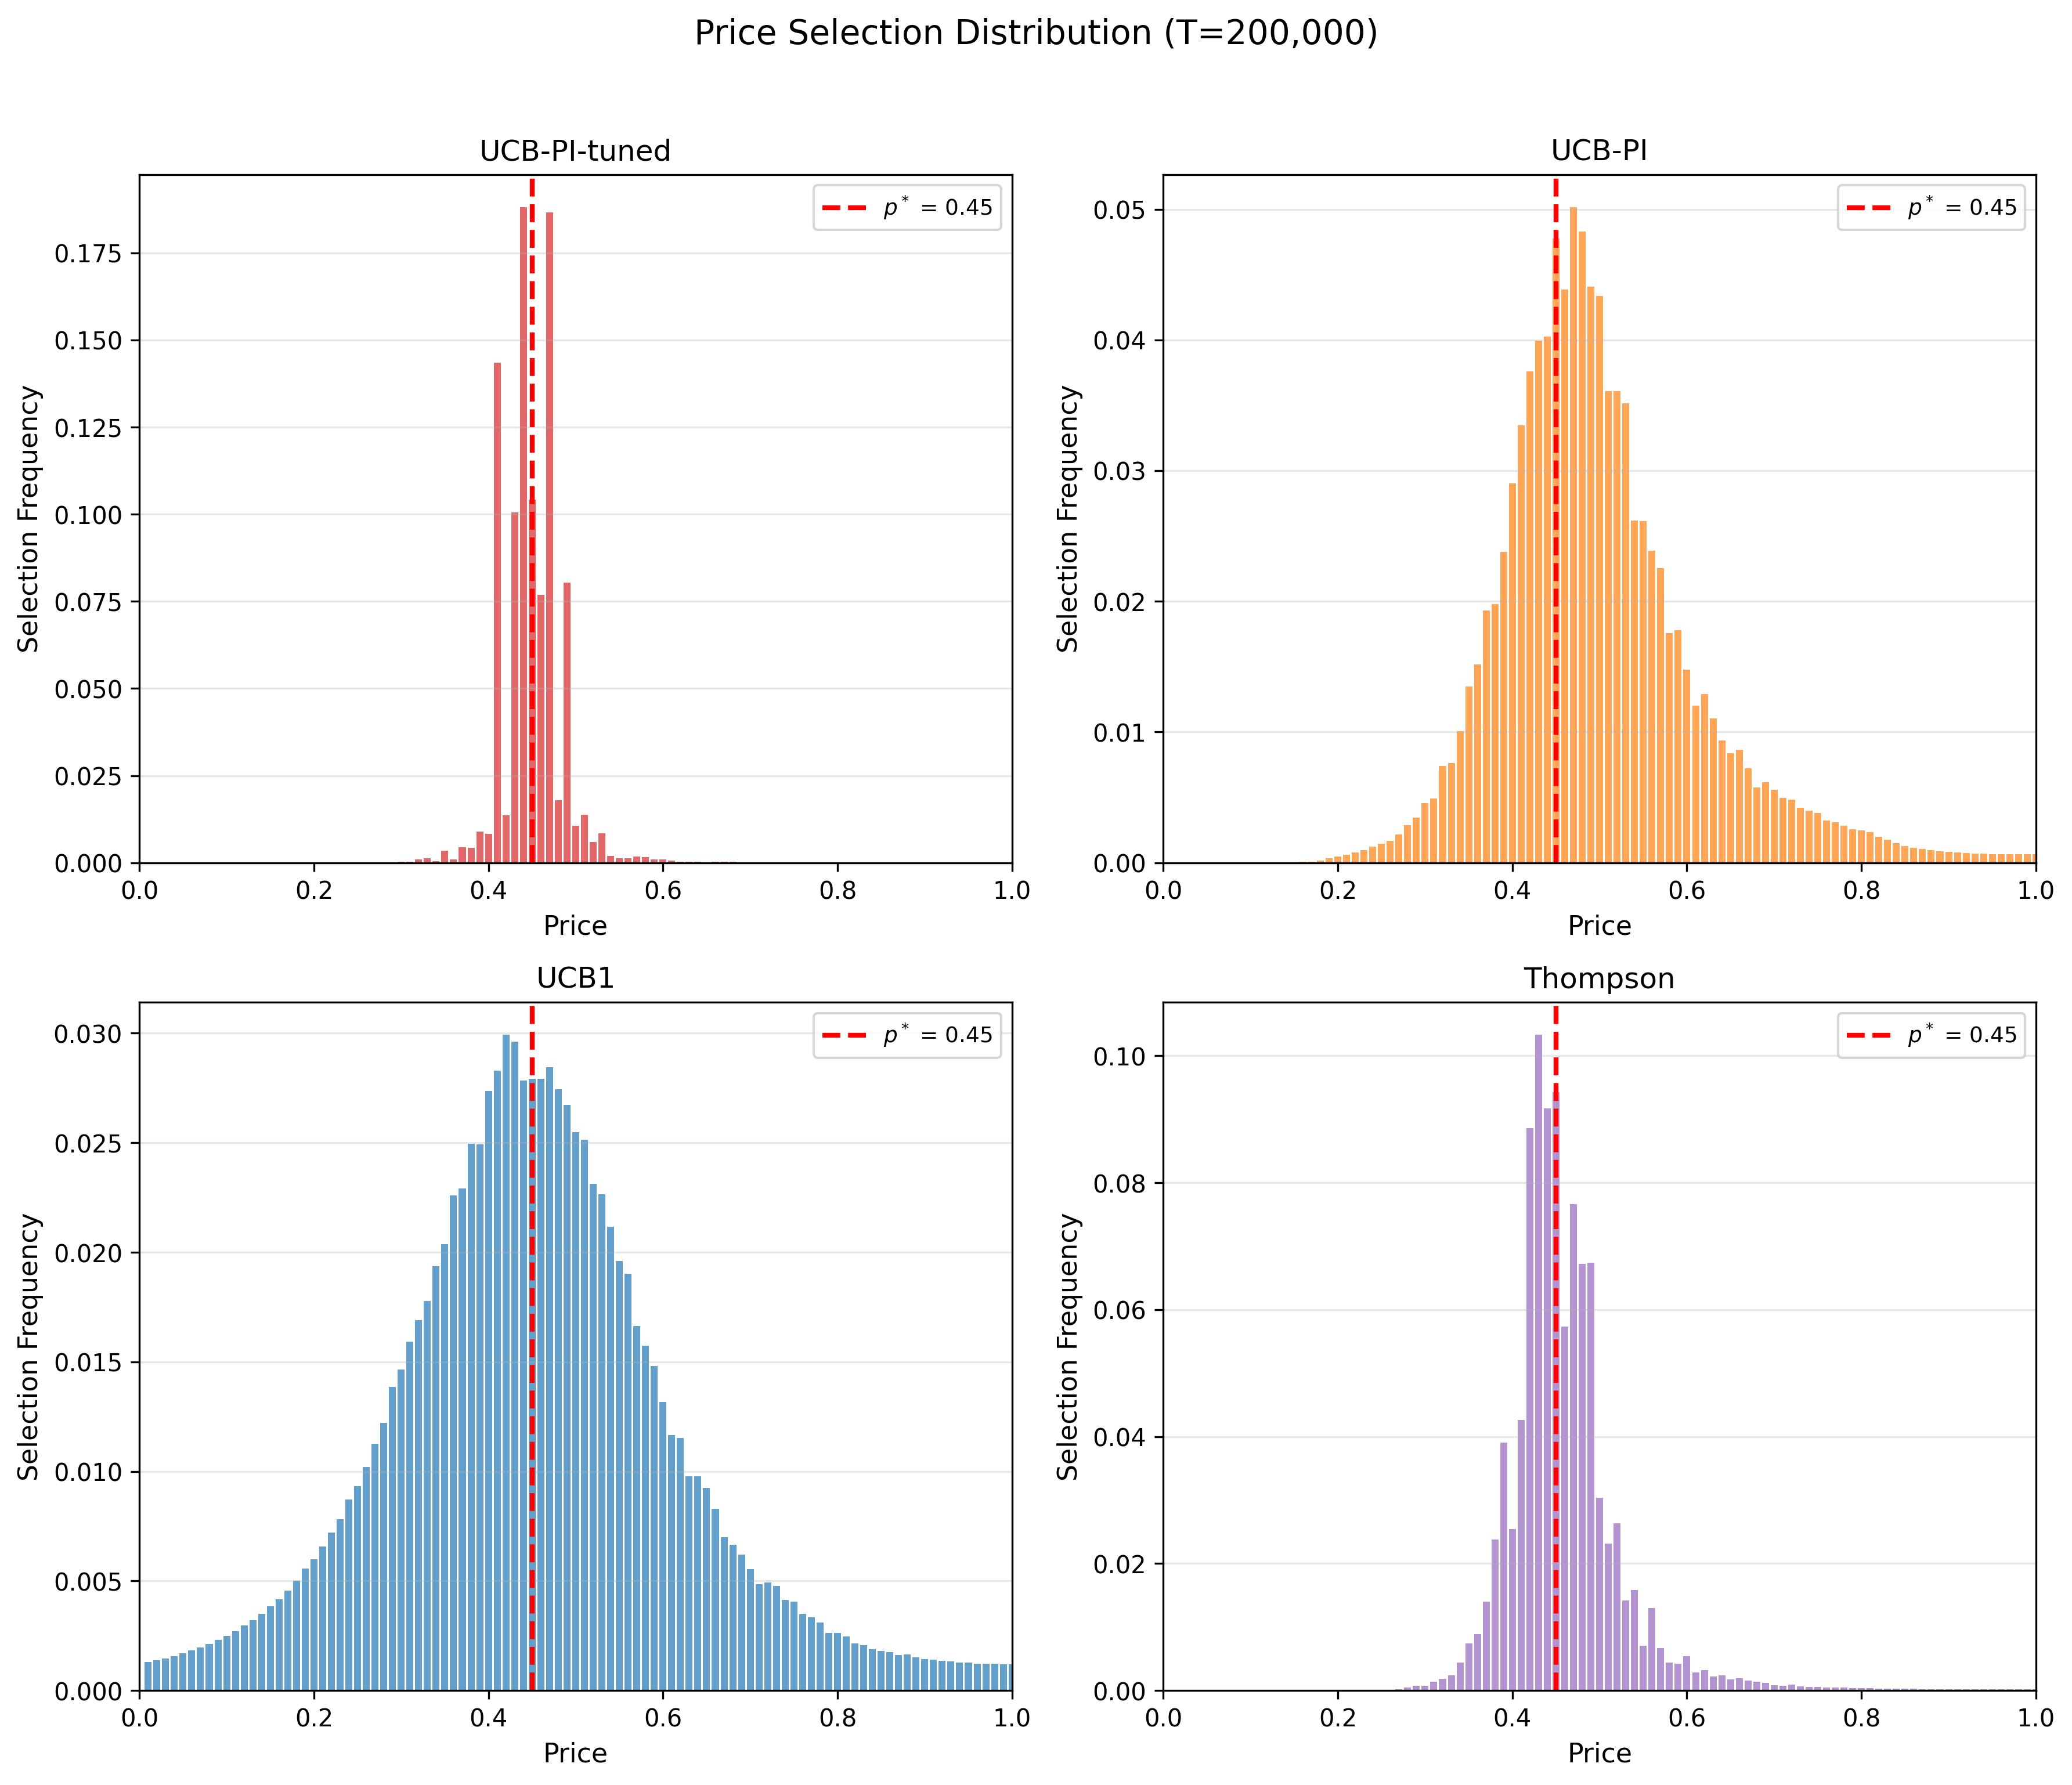
\includegraphics[width=0.9\textwidth]{../ch06_bandits/sims/structural_pricing_misra_price_histogram.png}
\caption{Price selection distribution by algorithm. Vertical dashed line marks optimal price $p^* = 0.45$.}
\label{fig:price_histogram}
\end{figure}

Figure~\ref{fig:convergence} shows the convergence trajectory using a moving average of the selected price. UCB-PI-tuned converges to near $p^*$ within the first 50{,}000 rounds and remains stable. The standard UCB-PI converges more slowly due to aggressive dominance that occasionally eliminates near-optimal prices early.

\begin{figure}[!htbp]
\centering
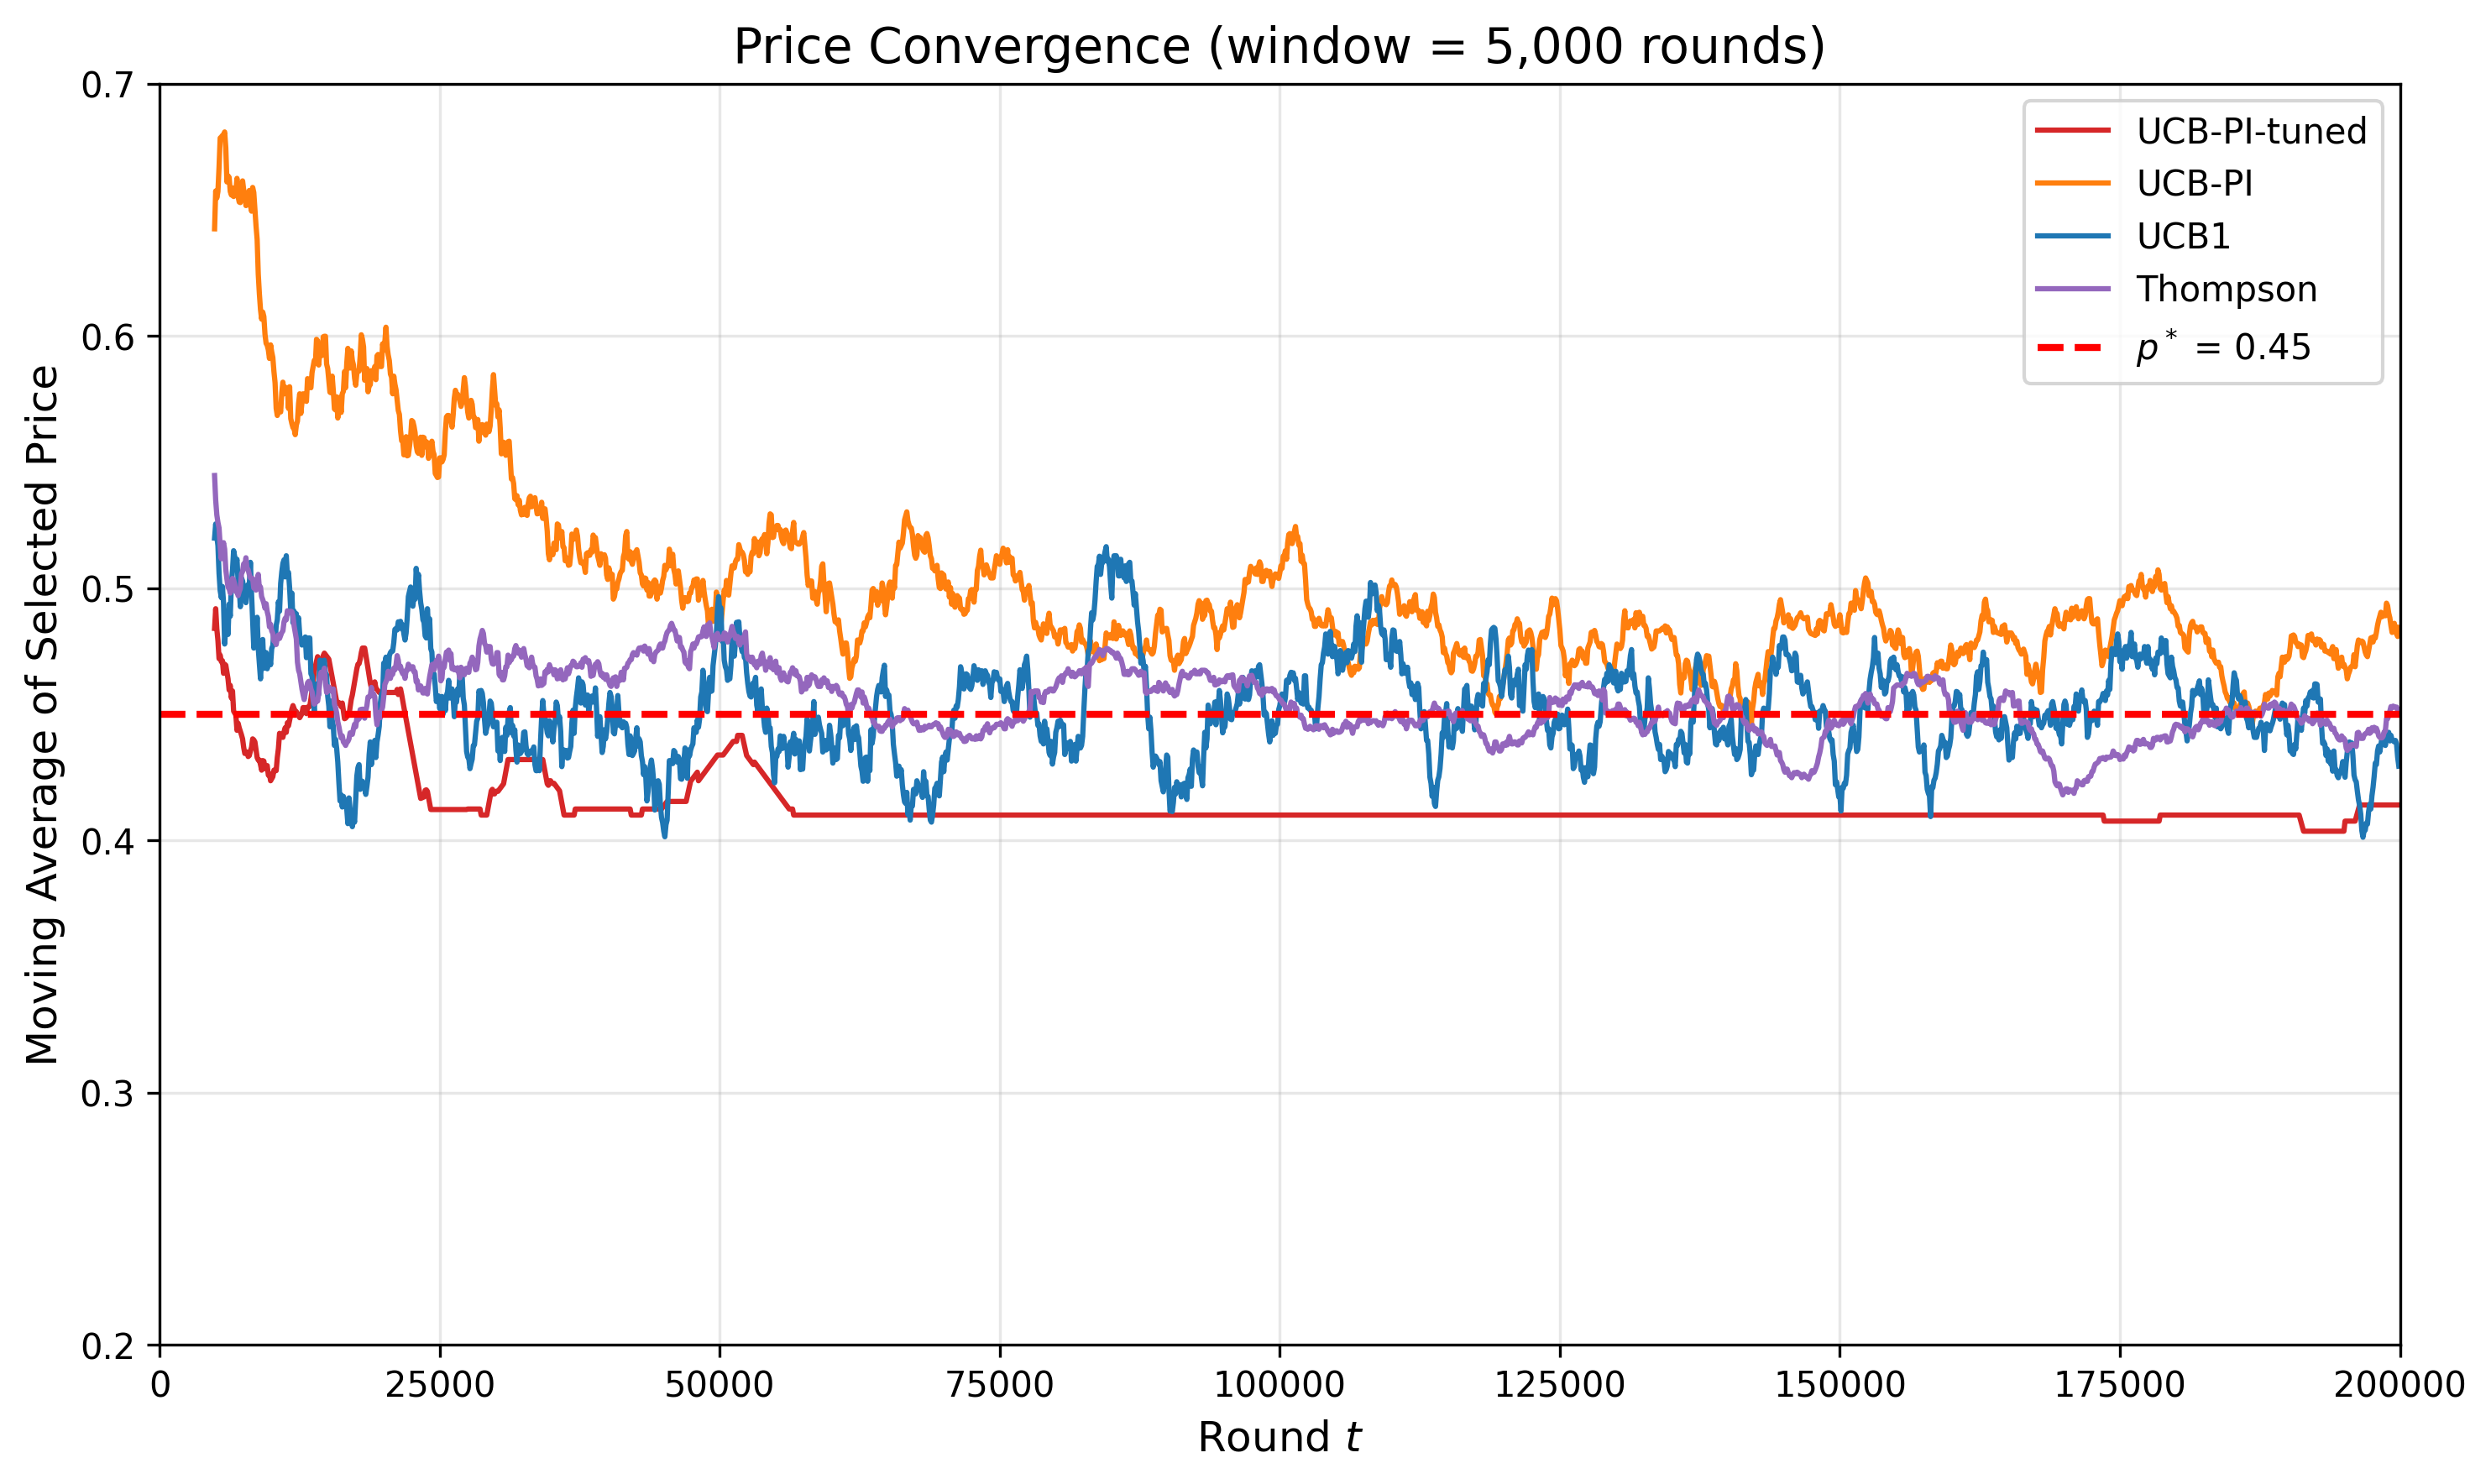
\includegraphics[width=0.9\textwidth]{../ch06_bandits/sims/structural_pricing_misra_convergence.png}
\caption{Convergence trajectory (moving average of selected price, window = 1000). Horizontal dashed line marks optimal price $p^* = 0.45$.}
\label{fig:convergence}
\end{figure}
